\section{CFD model}
    Během výpočtů byl použit předpoklad stacionárního vazkého proudění ideálního plynu, od čehož se odvíjela i forma níže uvedených rovnic. 
    \subsection{Základní systém rovnic}
        
        \subsubsection{Rovnice kontinuity}
            Zákon zachování hmotnosti je pro stlačitelné stacionární proudění popsán následující rovnicí:
            \begin{equation} \label{eq:rovnice-kontinuity}
                \nabla \cdot  \brac{\rho \Vec{u}} = 0  
            \end{equation}
            \noindent kde $\rho \unit{\frac{kg}{m^3}}$ je hustota a $\Vec{u} \unit{\frac{m}{s^2}}$  je rychlost proudění.
        
        \subsubsection{Pohybová rovnice}
            Přenos hybnosti je popsán Navier-Stokesovými rovnicemi pro stacionární proudění:
            \begin{equation} \label{eq:pohybova-rovnice}
                \nabla \cdot \brac{\rho \Vec{u} \otimes \Vec{u}} = - \nabla p + \nabla \cdot \Tensor{\tau} + \Vec{f}
            \end{equation}
            \noindent kde $p \unit{Pa}$ je statický tlak, $\Vec{f} \unit{\frac{N}{m^3}}$ je vektor vnějších sil a $\Tensor{\tau} \unit{\frac{N}{m^2}}$ je tenzor vazkých napětí daný následujícím vztahem:
            \begin{equation} \label{eq:tenzor-vazkych-napeti}
                \Tensor{\tau} = \mu \Brac{\nabla \Vec{u} + \nabla \Vec{u}^T - \frac{2}{3} \brac{\nabla \cdot \Vec{u}} I}
            \end{equation}
            \noindent kde $\mu \unit{Pa \cdot s}$ je dynamická viskozita a $I \unit{1}$ je jednotková matice.
            
        \subsubsection{Energetická rovnice}
            Řešení stlačitelného proudění vyžaduje doplnění energetické rovnice, kterou lze zapsat následovně:
            \begin{equation} \label{eq:energeticka-rovnice}
                \nabla \cdot \brac{\rho \Vec{u} H + \Vec{q} - \Tensor{\tau} \cdot \Vec{u}} = 0
            \end{equation}
            \noindent kde $H \unit{\frac{J}{kg}}$ je celková měrná entalpie a $\Vec{q} \unit{\frac{W}{m^2}}$ je vektor tepelného toku.
        \subsubsection{Konstitutivní vztahy}
        \smallSection{Stavová rovnice ideálního plynu}
        Rovnice popisuje vazbu mezi stavovými veličinami tekutiny:
        \begin{equation} \label{eq:stavova-rovnice}
            \frac{p}{\rho} = r T
        \end{equation}
        \noindent kde $T \unit{K}$ je termodynamická teplota a $r \unit{\frac{J}{kg \cdot K}}$ je měrná plynová konstanta, pro vzduch rovna $287.2 \unit{\frac{J}{kg \cdot K}}$.
        
        \smallSection{Celková měrná entalpie}
        Měrnou entalpii proudění $h \unit{\frac{J}{kg}}$ lze určit ze vztahu:
        \begin{equation} \label{eq:entalpie}
            h = c_p T = e + \frac{p}{\rho} = c_v T + \frac{p}{\rho}
        \end{equation}
        \noindent kde $c_p \, , \; c_v  \unit{\frac{J}{kg \cdot K}}$ jsou měrné tepelné kapacity za konstantního tlaku, resp. konstantního objemu a $e \unit{\frac{J}{kg}}$ je měrná energie. Přičtením měrné kinetické energie proudění dostáváme celkovou měrnou entalpii $H$:
        \begin{equation} \label{eq:celkova-entalpie}
            H = h + \frac{\norm{\Vec{u}}^2}{2}
        \end{equation}
        
    \subsection{Model turbulence}
        Pokračování – theory guide, s106, BSL
        \begin{align} \label{eq:rovnice-pro-k} 
            \nabla \cdot \brac{\rho k \Vec{u}} &= \nabla \cdot \brac{\Gamma _k \nabla k} + G _k - Y _k + S _k + G _b \\
            \Gamma _k &= \mu + \frac{\mu _t}{\sigma _k} \\
            \mu _t &= \alpha ^* \frac{\rho k}{\omega} \\
            \mu _t &= \alpha ^* \frac{\rho k}{\omega} \\
            \alpha ^* &= \alpha ^* _\infty \brac{\frac{\alpha _0 ^* + \frac{Re_t}{R_k}}{1 + \frac{Re_t}{R_k}}} \\
            Re_t &= \frac{\rho k}{\mu \omega} \\
            R_k &= 6 \\
            \alpha ^* _0 &= \frac{\beta _i}{3} \\
            G_k &= \mu _t S^2 \\
            S &= \sqrt{2 \Tensor{S} : \Tensor{S}} \\
            \Tensor{S} &= \frac{1}{2} \brac{\nabla \Vec{u} + \nabla \Vec{u} ^T} \\
            Y _k &= \rho \beta ^* f_{\beta ^*} k \omega \\
            f_{\beta ^*} &= \begin{cases} 
                1 & X_k \leq 0 \\
                \frac{1 + 680 X _k ^2}{1 + 400 X _k ^2} & X _k > 0 \\                
                \end{cases} \\
            X _k &= \frac{1}{\omega ^3} \nabla k \cdot \nabla \omega \\
            \beta ^* &= \beta ^* _i \Brac{1 + \zeta ^* F \brac{\Ma_t}} \\
            \beta _i ^* &= \beta _\infty ^* \Brac{\frac{\frac{4}{15} + \brac{\frac{Re_t}{R_\beta}}^4}{1 + \brac{\frac{Re_t}{R_\beta}}^4}}
        \end{align}

        \begin{align} \label{eq:rovnice-pro-omega}
            \nabla \cdot \brac{\rho \omega \Vec{u}} &= \nabla \cdot \brac{\Gamma _\omega \nabla \omega} + G _\omega - Y _\omega + S _\omega + G _{\omega b} \\
            \Gamma _\omega &= \mu + \frac{\mu _t}{\sigma _\omega} \\
            G _\omega &= \alpha \frac{\omega}{k} G _k \\
            \alpha &= \frac{\alpha _\infty}{\alpha ^*}\brac{\frac{\alpha _0 + \frac{Re_t}{R_\omega}}{1 + \frac{Re_t}{R_\omega}}} \\
            Y _\omega &= \rho \beta f_\beta \omega ^2 \\
            f _\beta &= \frac{1 + 70 X \omega}{1 + 80 X _\omega} \\
            X _\omega &= \left| \frac{\brac{\Tensor{\Omega} \cdot \Tensor{\Omega}} : \Tensor{S}}{\brac{\beta _\omega ^* \omega}^3} \right| \\
            \Tensor{\Omega} &= \frac{1}{2} \brac{\nabla \Vec{u} - \nabla \Vec{u}^T} \\
            \beta &= \beta _i \Brac{1 - \frac{\beta _i ^*}{\beta _i} \zeta ^* F\brac{\Ma_t}} \\
            F \brac{\Ma_t} &= \begin{cases}
                0   &   \Ma_t \leq \Ma_{t0} \\
                \Ma_t ^2 - \Ma _{t0} ^2 & \Ma_t > \Ma _{t0} \\
            \end{cases} \\
            \Ma _t ^2 &= \frac{2k}{a^2} \\
             a &= \sqrt{\kappa r T}
        \end{align}

        \begin{table}[ht!]
            \centering
            \begin{tabular}{l|l|l|l|l|l|l|l|l|l|l|l}
            $\alpha _\infty ^*$ & $\alpha _\infty$ & $\alpha _0$  & $\beta _\infty ^*$ & $\beta _i$ & $R_\beta $ & $R_k$ & $R_\omega$ & $\zeta ^*$ & $\Ma _{t0}$ & $\sigma _k$ & $\sigma _\omega$ \\ \hline
            $1$                 & $0.52$           & $\frac{1}{9} $& $0.09$             & $0.072$    & $8$        & $6$   & $2.95$     & $1.5$      & $0.25$      & $2$         & $2$             
            \end{tabular}
            \caption{Konstanty modelu k-$\omega$ SST.}
            \label{tab:konstanty-turbulence}
            \end{table}
    \newpage
    \subsection{Výpočetní geometrie}
        Vzhledem k charakteru řešeného problému byla geometrie proměnlivá. Jednotícím prvkem byla přítomnost alespoň jednoho ze dvou teplotních čidel, jehož restituční faktor byl zkoumán. Podle aktuální simulace se však měnilo uspořádání a přítomnost dalších geometrických prvků, jako například stínění.
    
        \subsubsection{Výpočetní oblast}
            Výpočty byly prováděny na geometrii umístěné v kontrolní oblasti tvaru válce o průměru $250 \Unit{mm}$ a délce $450 \Unit{mm}$. Vzhledem k rozměrům čidel, respektive celkové konstrukce, se jednalo o dostatečně velký kontrolní objem, který neměl ovlivňovat proudění okolo sondy. Veškeré měřené geometrie byly ve válci umístěné $100 \Unit{mm}$ od vstupní oblasti, viz obrázek \ref{fig:vypocetni-oblast}, ze kterého je patrné i umístění souřadného systému, na který bude dále v práci odkazováno.
            
            \begin{figure}[ht!]
                \centering
                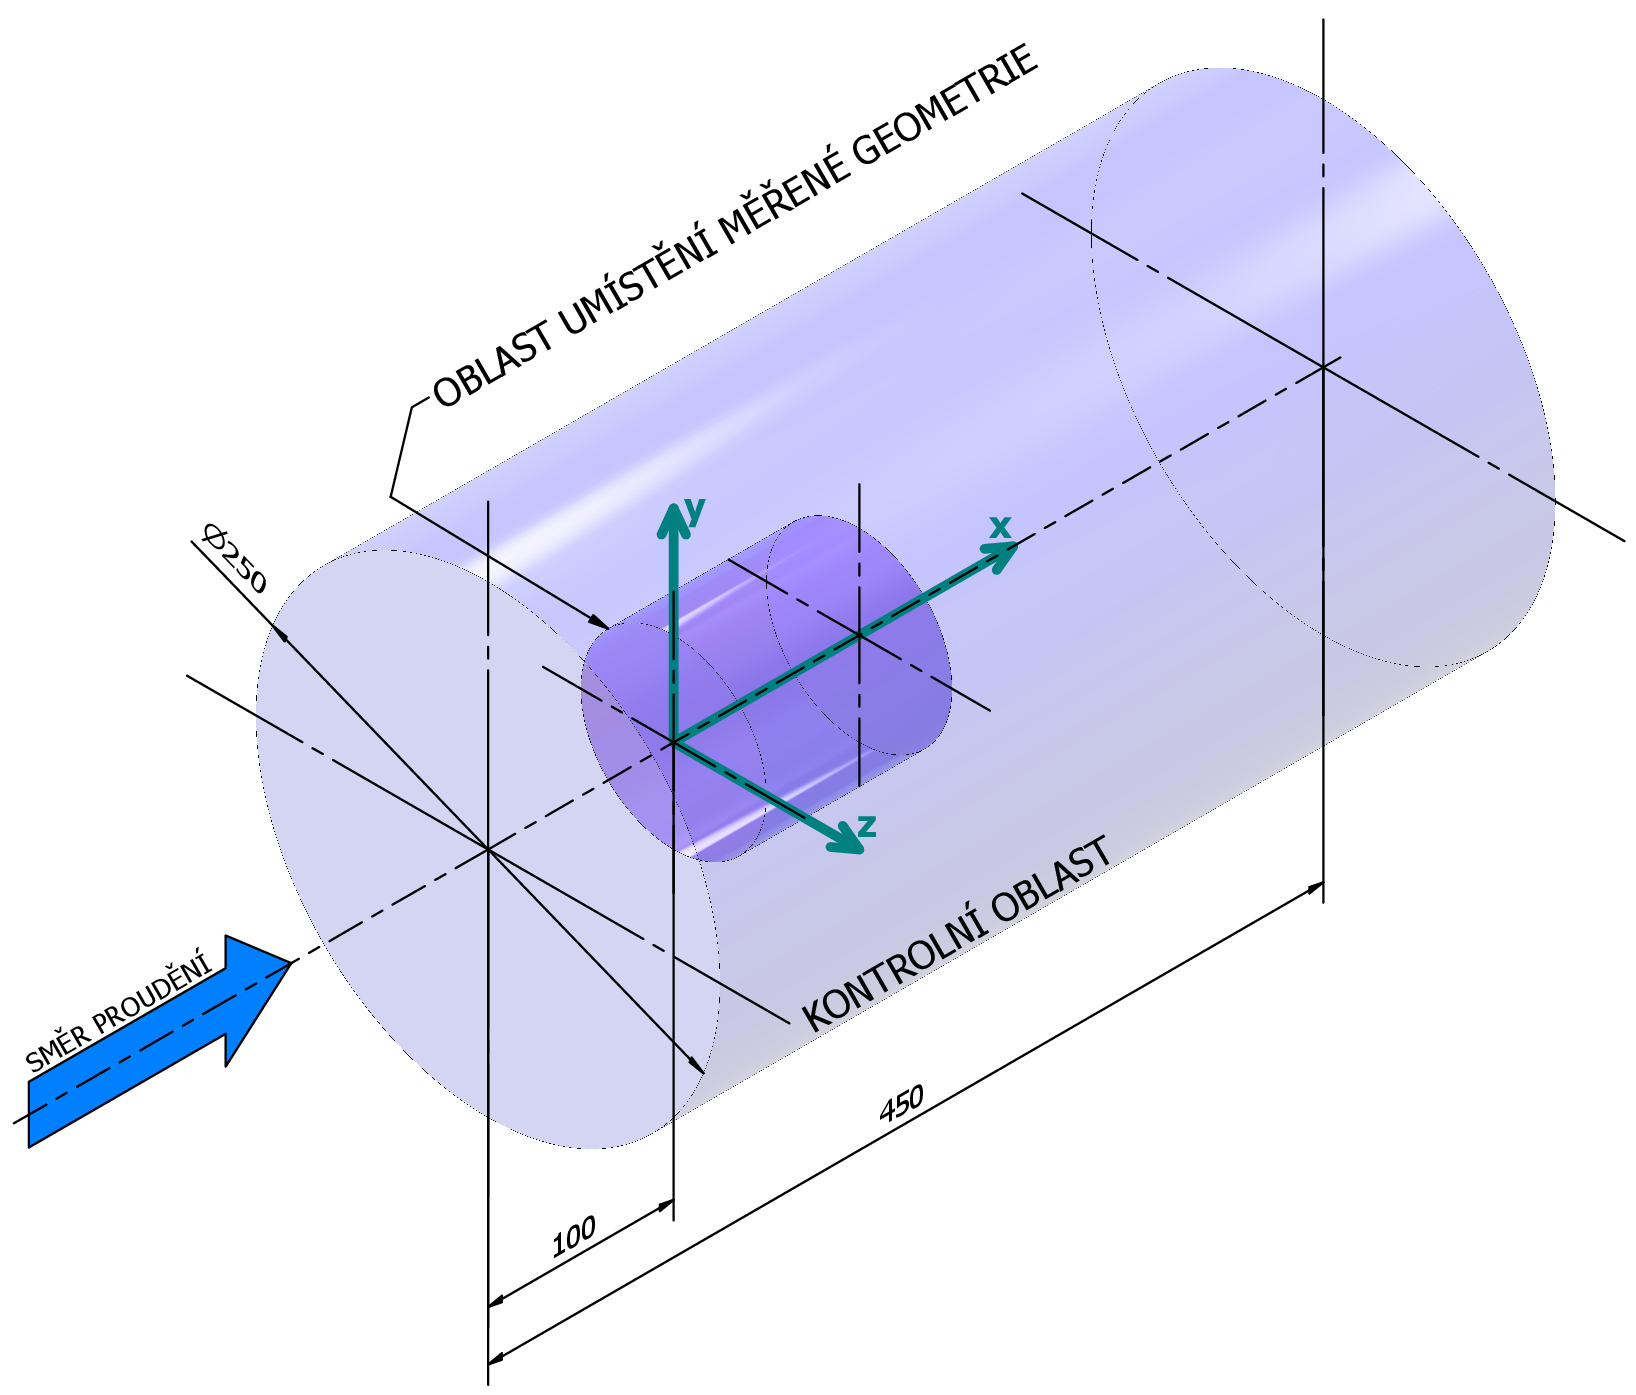
\includegraphics[width=\textwidth]{300_VYPOCETNI_MODEL/Vypocetni_oblast.png}
                \caption{Výpočetní oblast s vyznačením souřadného systému a polohy měřených geometrií.}
                \label{fig:vypocetni-oblast}
            \end{figure}
        
        \subsubsection{Využití symetrie}
            U všech zkoumaných geometrií se nacházela alespoň jedna rovina symetrie – bylo tedy možné využít této výhody pro úsporu výpočetního výkonu. Veškeré simulace uvedené v kapitolách \ref{sec:konstrukcni-upravy} a \ref{sec:finalni-geometrie} s výjimkou analýzy směrové citlivosti v rovině $XZ$ byly provedeny s využitím symetrie výpočetního modelu, viz obrázek \ref{fig:vypocetni-oblast-symetrie}.
            
            \begin{figure}[ht!]
                \centering
                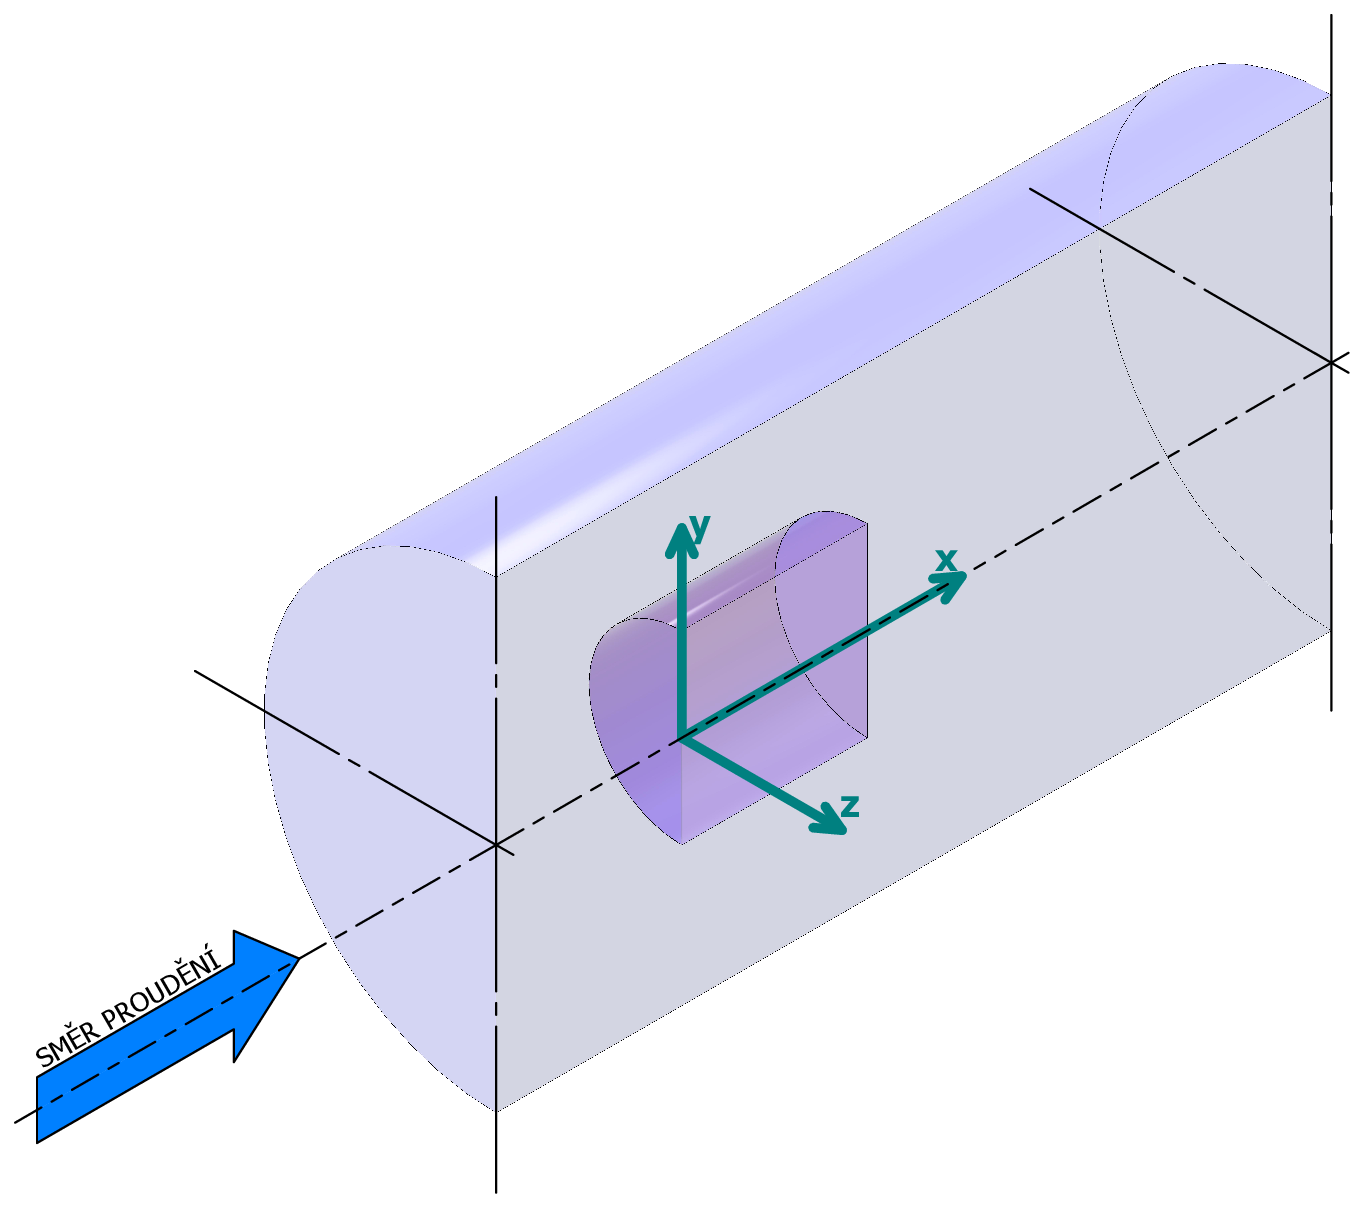
\includegraphics[width=\textwidth]{300_VYPOCETNI_MODEL/Vypocetni_oblast_symetrie.png}
                \caption{Výpočetní oblast pro řešení symetrických úloh.}
                \label{fig:vypocetni-oblast-symetrie}
            \end{figure}
         
	\newpage
        \subsubsection{Materiály}
            Během výpočtů byly uvažovány celkem tři materiály, ze kterých se skládala geometrie – trubice byla tvořena mosazí, čidla byla uvažována jako homogenní tělesa z keramiky $Al_2 O_3$ a těsnění bylo reprezentováno pryží. Použité fyzikální vlastnosti jednotlivých materiálů jsou uvedeny v tabulce \ref{tab:materialy}.
            
            \renewcommand{\arraystretch}{2}
            \begin{table}[ht!]
                \centering
                %\resizebox{.7\textwidth}{!}{%
                \begin{tabular}{l|l|l|l}
                                                                                  & Mosaz                        & Pryž                        &  Keramika                      \\ \hline
                    Hustota $\unit{\frac{kg}{m^3}}$                               & \multicolumn{1}{c|}{$8730$}  & \multicolumn{1}{c|}{$1100$} & \multicolumn{1}{c}{$3500$}     \\ \hline
                    Měrná tepelná kapacita $\unit{\frac{J}{kg \cdot K}}$          & \multicolumn{1}{c|}{$400$}   & \multicolumn{1}{c|}{$1300$} & \multicolumn{1}{c}{$700$}      \\ \hline
                    Tepelná vodivost $\unit{\frac{W}{m \cdot K}}$                 & \multicolumn{1}{c|}{$96$}    & \multicolumn{1}{c|}{$0.09$} & \multicolumn{1}{c}{$30$}      
                \end{tabular}%
                %}
                \caption{Fyzikální vlastnosti použitých materiálů.}
                \label{tab:materialy}
            \end{table}
            
            Jako proudící médium byl uvažován vzduch splňující stavovou rovnici ideální plynu (viz vztah \ref{eq:stavova-rovnice}) s následujícími vlastnostmi:

		\begin{table}[ht!]
			\centering
			%\resizebox{.7\textwidth}{!}{%
			\begin{tabular}{l|l}
				Měrná plynová konstanta $\unit{\frac{J}{kg \cdot K}}$ & Poissonovo číslo $\unit{1}$ \\ \hline
				\multicolumn{1}{c|}{$287$}                                                                        & \multicolumn{1}{c}{$1.4$}                \\ \hline
				Tepelná vodivost $\unit{\frac{W}{m \cdot K}}$ & Dynamická viskozita $\unit{Pa \cdot s}$ \\ \hline				
				\multicolumn{1}{c|}{$2.42 \cdot 10^{-2}$}                          &  \multicolumn{1}{c}{$1.7894 \cdot 10^{-05}$}     
			\end{tabular}%
			%}
			\caption{Fyzikální vlastnosti vzduchu.}
			\label{tab:vzduch}
		\end{table}
            
            
     \newpage      
    \subsection{Okrajové podmínky}
        \subsubsection{Hranice výpočetní oblasti}
			Hranice válcové kontrolní oblasti byla rozdělena na tři části s odlišnými okrajovými podmínkami – podstavy válce představovaly vstup a výstup a jeho plášť poté nenarušený proud (viz obrázek \ref{fig:okrajove-podminky}). Ve všech oblastech byly předepsány hodnoty uvedené v tabulce \ref{tab:spolecne-op}. Ve vstupní oblasti byla dále zadávána rychlost proudění, respektive velikost vektoru rychlosti a jeho směrové cosiny (využito při analýze směrové citlivosti). Hranice nenarušeného proudu měla předepisovánu hodnotu Machova čísla a směr proudění (opět ve formě směrových cosinů vektoru rychlosti). 

	     \begin{figure}[ht!]
                    \centering
                        \begin{subfigure}{0.3\textwidth}
                             \centering
                             \captionsetup{width=.9\linewidth}
                                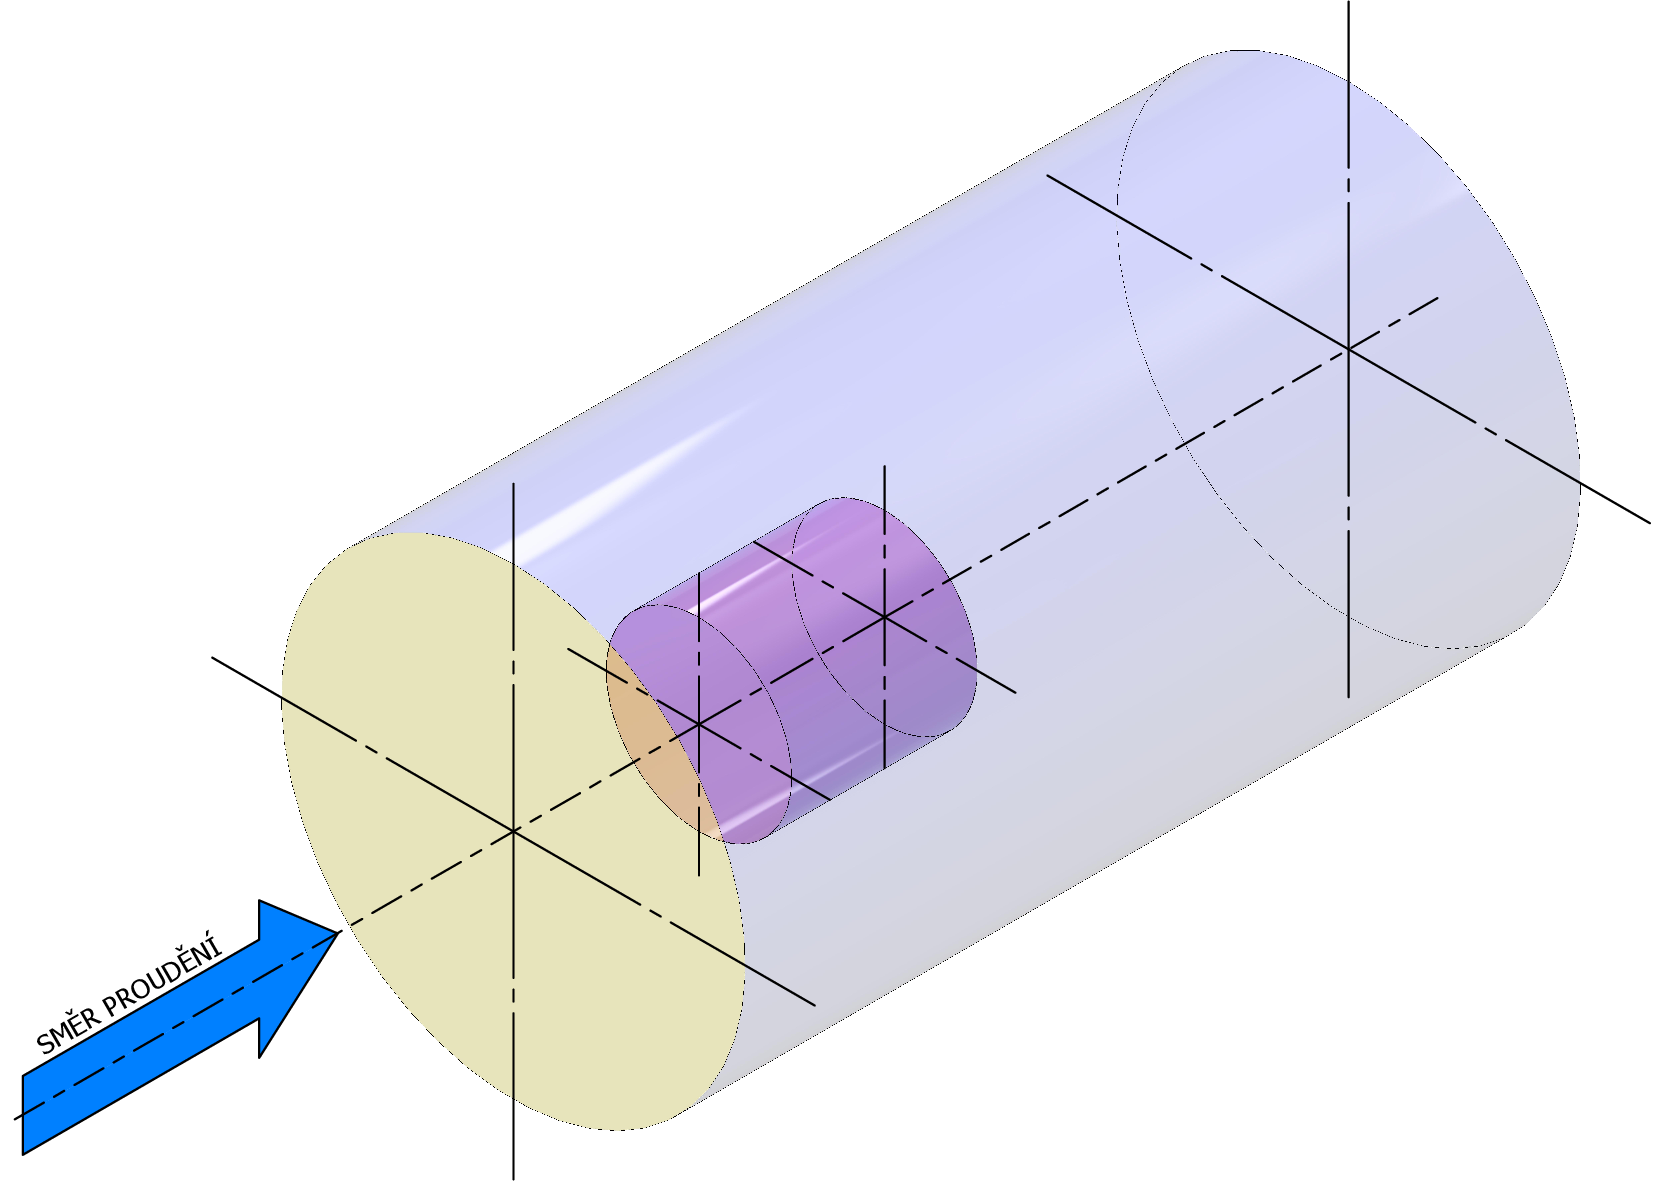
\includegraphics[width=\textwidth]{300_VYPOCETNI_MODEL/op-inlet.png}
                             \caption{Vstupní oblast.}
                             \label{fig:inlet}
                         \end{subfigure}
                         \begin{subfigure}{0.3\textwidth}
                             \centering
                             \captionsetup{width=.9\linewidth}
                             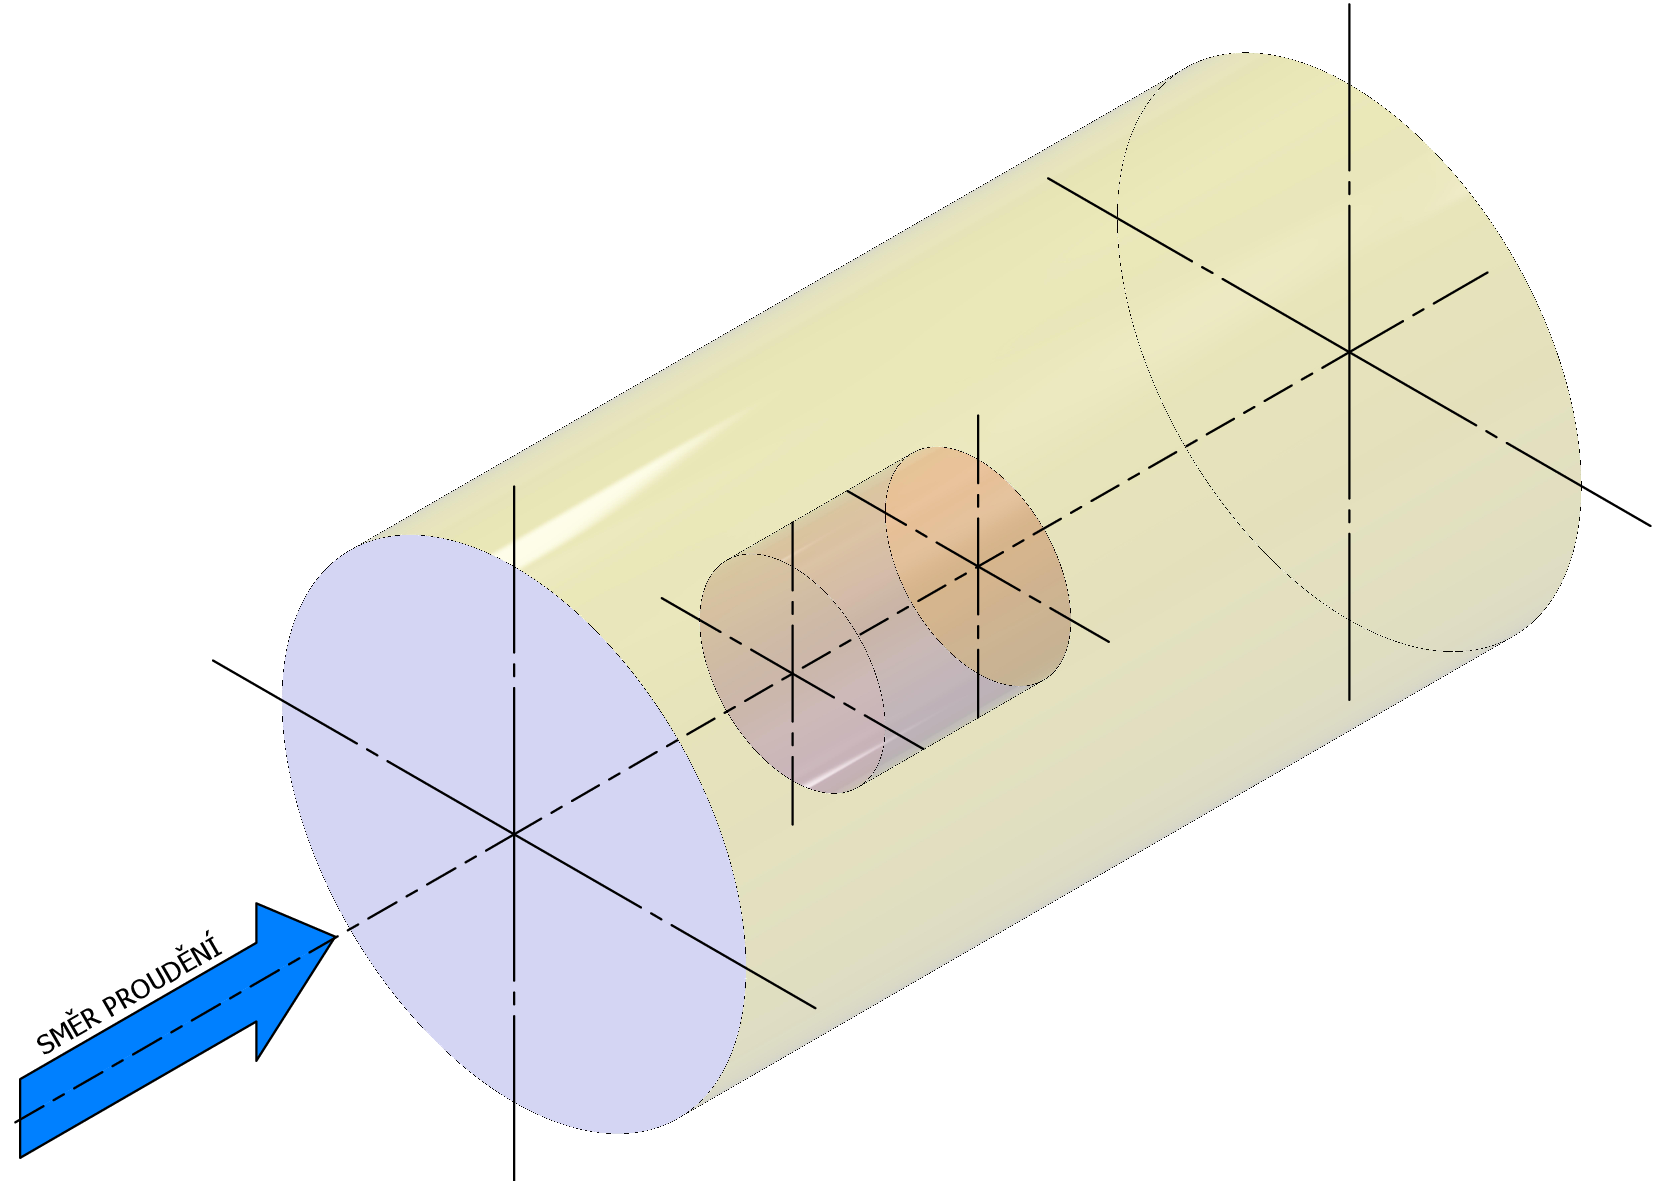
\includegraphics[width=\textwidth]{300_VYPOCETNI_MODEL/op-farfield.png}
                             \caption{Nenarušený proud.}
                             \label{fig:farfield}
                         \end{subfigure}
					\begin{subfigure}{0.3\textwidth}
                             \centering
                             \captionsetup{width=.9\linewidth}
                             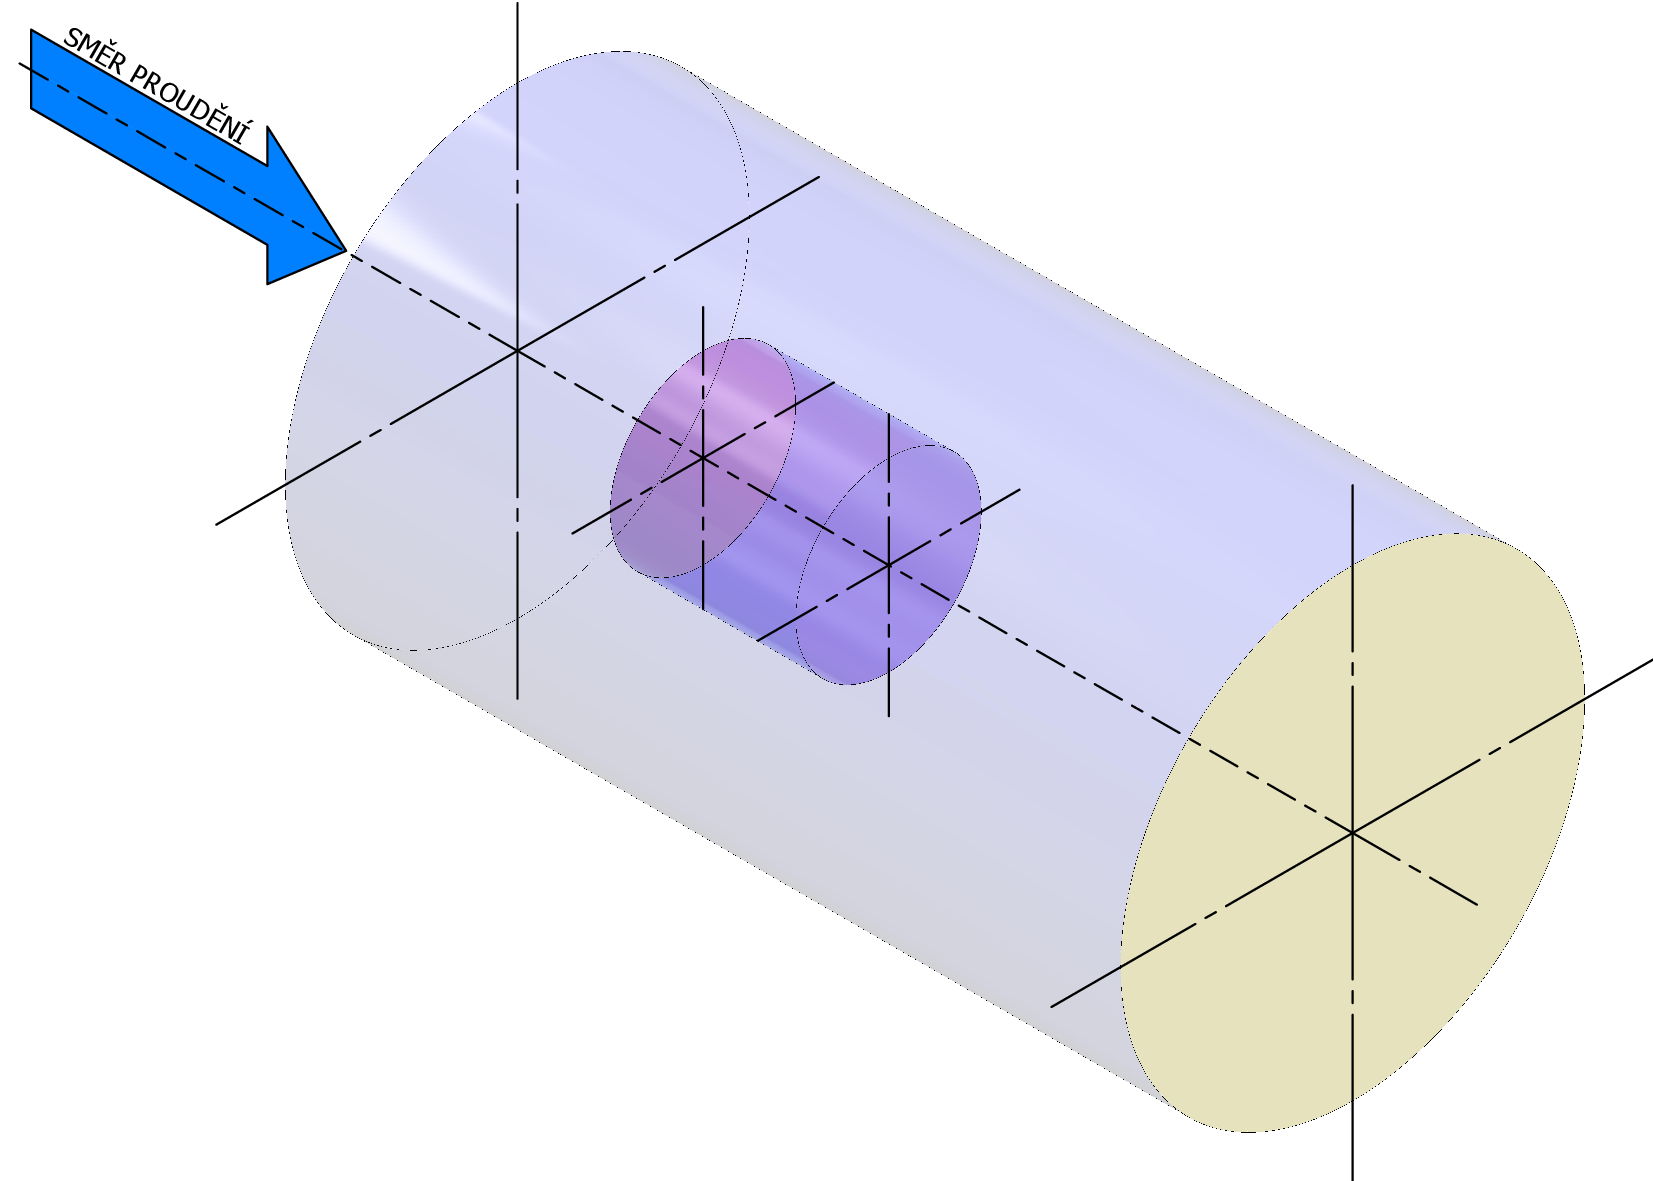
\includegraphics[width=\textwidth]{300_VYPOCETNI_MODEL/op-outlet.png}
                             \caption{Výstupní oblast.}
                             \label{fig:outlet}
                         \end{subfigure}
                    \caption{Části hranice pro aplikování okrajových podmínek (v jednotlivých obrázcích označeny žlutou barvou).}
                    \label{fig:okrajove-podminky}
         \end{figure}

         \begin{table}[ht!]
            \centering
            %\resizebox{.7\textwidth}{!}$ & Směšovací délka $\unit{m}$  \\ \hline
                \multicolumn{1}{c|}{2.5}         & \multicolumn{1}{c}{0.01}   
            \end{tabular}%
            %}
            \caption{Hodnoty předepisované na hranici kontrolní oblasti.}
            \label{tab:spolecne-op}
        \end{table}

         Výchozí rychlostí použitou pro testování bylo $250 \Unit{\frac{m}{s}}$, tomu odpovídá při teplotě $300 \Unit{K}$ Machovo číslo $0.72$. Nebude-li dále uvedeno jinak, pak byly pro výpočet použity právě tyto hodnoty.
			
        
        \subsubsection{Stěny}
            Při numerických simulacích bylo pro vyhodnocení restitučních faktorů třeba počítat s přestupem tepla do pevných látek a s jeho šířením objemem. V místech kontaktu proudícího média se stěnami geometrie byla proto použita podmínka sdílené teploty – teplota na hranici tekutiny byla přenesena na hranici tělesa.

    \newpage
    \subsection{Výpočetní síť} \label{sec:vypocetni-sit}
        Vytváření modelů probíhalo v prostředí software Autodesk Inventor (verze 2021 a 2022), odkud byly následně vyexportovány ve formátu \textit{.dwg}. K přípravě pro síťování byl následně použit software Ansys SpaceClaim (verze 2020b-2021b), jehož účel spočíval primárně ve sdílení topologie modelu, vytváření jmenných sekcí a exportu do optimalizovaného formátu \textit{.pmdb}. Samotné síťování poté probíhalo v software Ansys Fluent (verze 2020b-2021b).
        \subsubsection{Povrchová síť}
            Prvním krokem při vytváření výpočetní sítě pro řešič bylo importování geometrie (soubor \textit{.pmdb}) a vysíťování jejích ploch pomocí triangulace. Zde bylo použito následující nastavení:

            \begin{table}[ht!]
                \centering
                \begin{tabular}{l|l}
                    $\frac{\textrm{Minimální}}{\textrm{Maximální}}$ velikost elementů $\unit{mm}$                                            & Poměrný růst velikosti elementů $\unit{1}$ \\ \hline
                    \multicolumn{1}{c|}{$\frac{0.1}{15}$}                                                              & \multicolumn{1}{c}{$1.2$}                  \\ \hline
                    Maximální úhel překlenutí $\unit{deg}$                                                         & Minimální dělení hran $\unit{1}$           \\ \hline
                    \multicolumn{1}{c|}{$10$}                                                                      & \multicolumn{1}{c}{$3$}                     
                \end{tabular}
                \caption{Předepisované hodnoty při vytváření povrchové sítě.}
                \label{tab:povrchova-sit-nastaveni}
            \end{table}

            Kvalita povrchové sítě byla následně kontrolována, aby šikmost žádného elementu nepřesáhla $0.5$. Šikmost představuje odchylku geometrie buňky od optimálního tvaru (v případě triangulace se jedná o rovnostranný trojúhelník). Její hodnota se pohybuje mezi $0 \div 1$, kde $0$ odpovídá nejlepší kvalitě. Pro správný průběh a konvergenci výpočtů je doporučeno, aby maximální šikmost nepřesahovala $0.95$ a aby se průměrná šikmost pohybovala nejvýše okolo hodnoty $0.33$ \cite{Ansys2020User}. Tato doporučení platí pro konečnou objemovou síť, která se používá během výpočtů, nicméně počáteční kvalita povrchové sítě má zásadní vliv na jakost následujícího síťování.
        \subsubsection{Zjemnění v mezní vrstvě}
            Pro dosažení přijatelné přesnosti výpočtu přestupu tepla ze vzduchu do těles bylo třeba vytvořit dostatečně jemnou síť v oblasti mezní vrstvy. K tomu byly využity prismatické buňky v místech kontaktu tekutiny s měřenou geometrií. Cílem bylo dosažení průměrné bezrozměrné vzdálenosti od stěny co nejblíže $1$. Toho bylo docíleno pomocí natavení uvedeného v tabulce \ref{tab:mezni-vrstva-nastaveni}. Příklad rozložení $y_+$ u teplotního čidla je uveden na obrázku \ref{fig:yplus-stineni-A}.

            \begin{table}[ht!]
                \centering
                \begin{tabular}{ll}
                    \multicolumn{2}{l}{Míra natažení prvního elementu (aspect ratio) $\unit{1}$}                            \\ \hline
                    \multicolumn{2}{c}{$6.2$}                                                                        \\ \hline
                    \multicolumn{1}{l|}{Poměrný růst velikosti elementů $\unit{1}$} & Počet prismatických vrstev $\unit{1}$ \\ \hline
                    \multicolumn{1}{c|}{$1.2$}                                      & \multicolumn{1}{c}{$10$}                
                \end{tabular}
                \caption{Předepisované hodnoty při vytváření prismatických buněk.}
                \label{tab:mezni-vrstva-nastaveni}
            \end{table}

            \begin{figure}[ht!]
                \centering
                \includegraphics*[width=\textwidth  ]{300_VYPOCETNI_MODEL/yplus-stineni-A.eps}
                \caption{Graf četností hodnot bezrozměrné vzdálenosti od stěny čidla A pro úlohu z kapitoly \ref{sec:stineni-A}. Průměrná hodnota je pro tento případ rovna $0.945$.}
                \label{fig:yplus-stineni-A}
            \end{figure}

            \newpage


        \subsubsection{Objemová síť}

        Při vytváření objemové sítě byly zvoleny polyhedrální buňky, které umožňují dosahovat přesnějších řešení oproti starším typům elementů při shodných počtech buňek. Umožňují navíc lepší odhad gradientu díky vyššímu počtu stěn a obecně lze s jejich použitím dosahovat lepší kvality sítě \cite{Sosnowski2018}. Postup generování objemové sítě byl následující:

        \begin{enumerate}
            \item Konverze povrchové triangulace na polygonální síť
            \item Vygenerování vrstev prismatických buněk
            \item Iterační generování polyhedrální objemové sítě ve zbytku objemu
        \end{enumerate}

        Maximální šikmost hotové sítě se vždy pohybovala pod hodnotou $0.85$. Počty buňek se pohybovaly v rozmezí $450 \div 550$ tisíc pro symetrické úlohy a $850 \div 950$ tisíc pro úlohy bez využití symetrie. Příklad výpočetní sítě je uveden na obrázku \ref{fig:sit-detail-stineni-A}.

        \begin{figure}
            \centering
            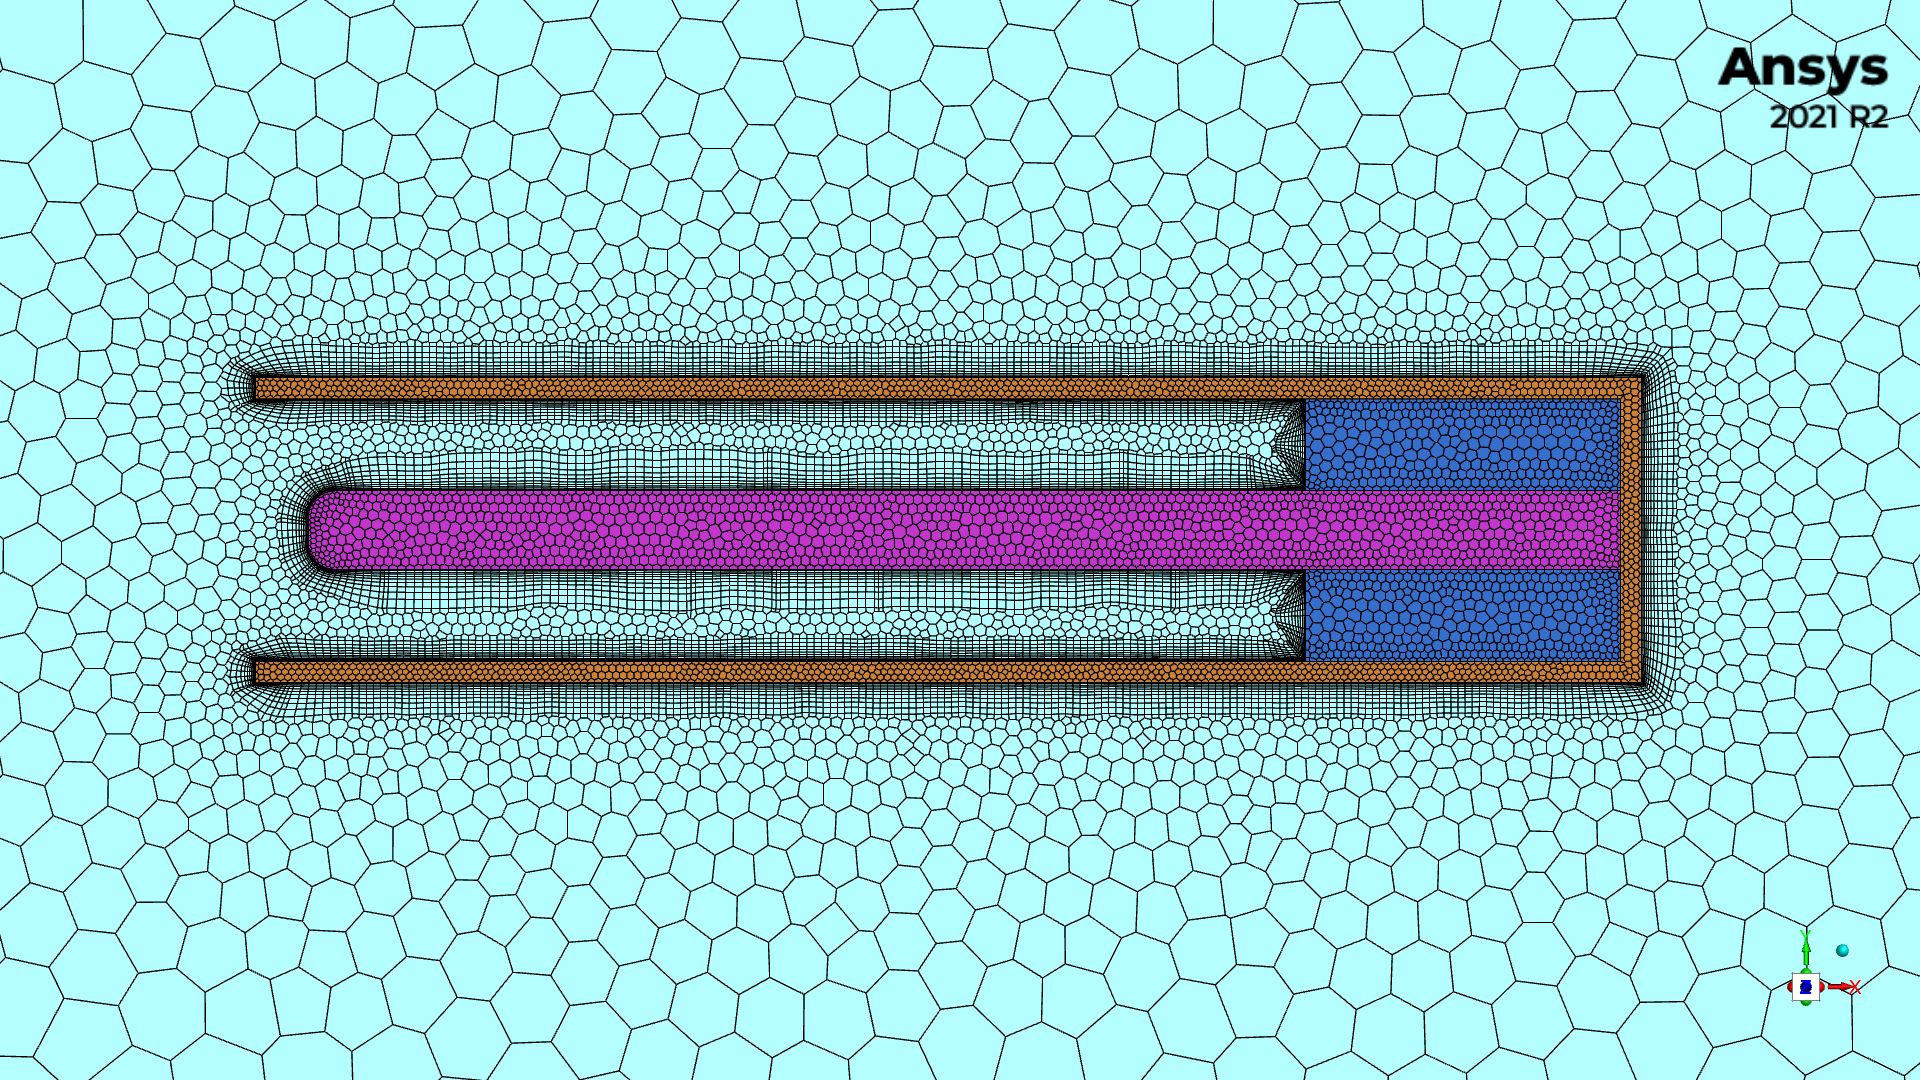
\includegraphics[width=\textwidth]{300_VYPOCETNI_MODEL/mesh_sym_odvetrani_A.png}
            \caption{Pohled na výpočetní síť z kapitoly \ref{sec:stineni-A} ze strany symetrie.}
            \label{fig:sit-detail-stineni-A}
        \end{figure}
        
    \subsection{Numerický řešič}
        \subsubsection{Metoda konečných objemů}
        \subsubsection{Odhad gradientu}
        \subsubsection{Aproximace hodnot na stěnách}
        \subsubsection{Numerické schéma}
        \subsubsection{Určení restitučních faktorů}

        
        